%% =============================================================================
\section{How to use this template}
\label{sec:example}


%% -----------------------------------------------------------------------------
\subsection{Citations}

\begin{itemize}

    \item
    You probably want to usually cite another source in a footnote like this\footnote{
        \citet{1905.Einstein.photoelectric-effect}.
    },
    and use \verb$\citet{X}$ within the footnote to refer to the author directly with only the date in parentheses.

    \item
    Or you can use \verb$\citet{X}$ to refer to the author directly in the inline text, again with only the date in parentheses:
    \citet{1905.Einstein.photoelectric-effect} defends the hypothesis that radiation is quantized.

    \item
    When citing the work at the end of a caption, you probably want to
    use \verb$\citep{X}$ to wrap the entire citation in parentheses:
    Steven Weinberg did foundational work forming the
    Standard Model~\citep{1967.Weinberg.A_model_of_leptons}.

    \item
    Probably fancier than necessary if using footnotes,
    but one can use \verb$\citep[see][]{X}$ to insert words in the citation:
    SUSY helps relax fine-tuning~\citep[see][]{1997.Martin.SUSY-primer}.
    There are some important papers in this
    world~\citep[\emph{e.g.}][]{1905.Einstein.photoelectric-effect}.

\end{itemize}


%% -----------------------------------------------------------------------------
\subsection{URLs}

This is an example url: \href{http://plato.stanford.edu/entries/structural-realism/}{Structural Realism}.
Or, you can put the text of the link in the document directly:
\url{http://plato.stanford.edu/entries/structural-realism/}.


%% -----------------------------------------------------------------------------
\subsection{Figures}

Blah blah blah. See \cref{fig:example/Martin-SUSY-running-of-couplings}.
And see \cref{tab:ATLAS-channels-per-sub-detector}.

Lorem ipsum dolor sit amet, consectetur adipisicing elit, sed do eiusmod tempor
incididunt ut labore et dolore magna aliqua. Ut enim ad minim veniam, quis
nostrud exercitation ullamco laboris nisi ut aliquip ex ea commodo consequat.
Duis aute irure dolor in reprehenderit in voluptate velit esse cillum dolore
eu fugiat nulla pariatur. Excepteur sint occaecat cupidatat non proident, sunt
in culpa qui officia deserunt mollit anim id est laborum.

%% example figure:

\begin{figure}[tp]
    \centering
    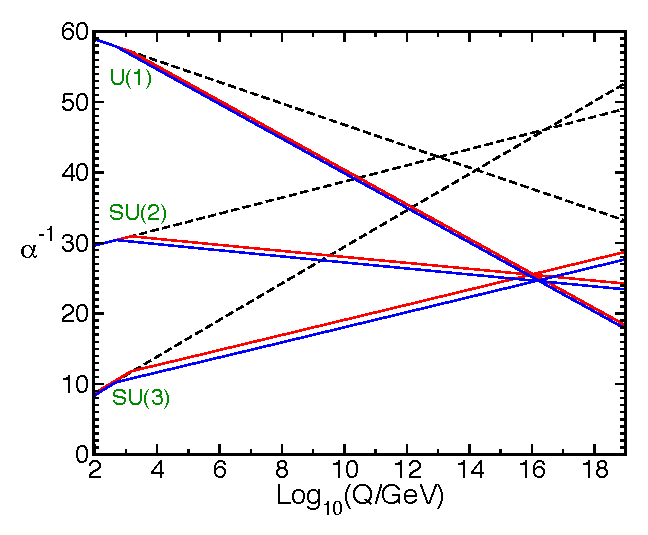
\includegraphics[width=0.70\textwidth]{figs/example/Martin-SUSY-running-of-couplings}
    \caption{
        Two-loop renormalization group evolution of the inverse
        gauge couplings $\alpha^{-1}(Q)$ in the Standard Model (dashed lines)
        and the Minimal Supersymmetric Standard Model  (MSSM, solid lines).
        In the MSSM case, the sparticle masses are treated as a common threshold varied
        between 500 GeV~(blue) and 1.5 TeV~(red)~\citep{1997.Martin.SUSY-primer}.
%        ~\cite{2003.deBoer.coupling-unification}.
    }   
    \label{fig:example/Martin-SUSY-running-of-couplings}
\end{figure}

%% example table:

\begin{table}[bp]
    \centering
    \caption{
        Number of readout channels per sub-detector in ATLAS for the primary sub-detectors
        (ignoring the minbias trigger system, luminosity monitors,
        and DCS sensors)~\citep{2008.ATLAS.detector-paper}.
    }
    \begin{tabular}{l l r}
        \hline\hline
        inner detector        &  Pixels            &   80 M \\
                              &  SCT               &  6.3 M \\ 
                              &  TRT               &  350 k \\ 
        \hline                     
        EM calorimeter        &  LAr barrel        &  110 k \\
                              &  LAr end-cap       &   64 k \\ 
        \hline                     
        hadronic calorimeter  &  tile barrel       &  9.8 k \\
                              &  LAr end-cap       &  5.6 k \\ 
                              &  LAr forward calo. &  3.5 k \\ 
        \hline                     
        muon spectrometer     &  MDTs              &  350 k \\
                              &  CSCs              &   31 k \\ 
                              &  RPCs              &  370 k \\ 
                              &  TGCs              &  320 k \\ 
        \hline                     
        total                 &                    &   88 M \\
        \hline\hline               
    \end{tabular}
    \label{tab:ATLAS-channels-per-sub-detector}
\end{table}


%% -----------------------------------------------------------------------------
\clearpage
\subsection{Wrapfig}

Lorem ipsum dolor sit amet, consectetur adipisicing elit, sed do eiusmod tempor
incididunt ut labore et dolore magna aliqua. Ut enim ad minim veniam, quis
nostrud exercitation ullamco laboris nisi ut aliquip ex ea commodo consequat.
Duis aute irure dolor in reprehenderit in voluptate velit esse cillum dolore
eu fugiat nulla pariatur. Excepteur sint occaecat cupidatat non proident, sunt
in culpa qui officia deserunt mollit anim id est laborum.

%% An example of using wrapfigure to wrap text around a figure.
%% Note that this figure does not "float" but stays right here.

\begin{wrapfigure}{r}{0.5\textwidth}
    \vspace{-0.3cm}
    \centering
    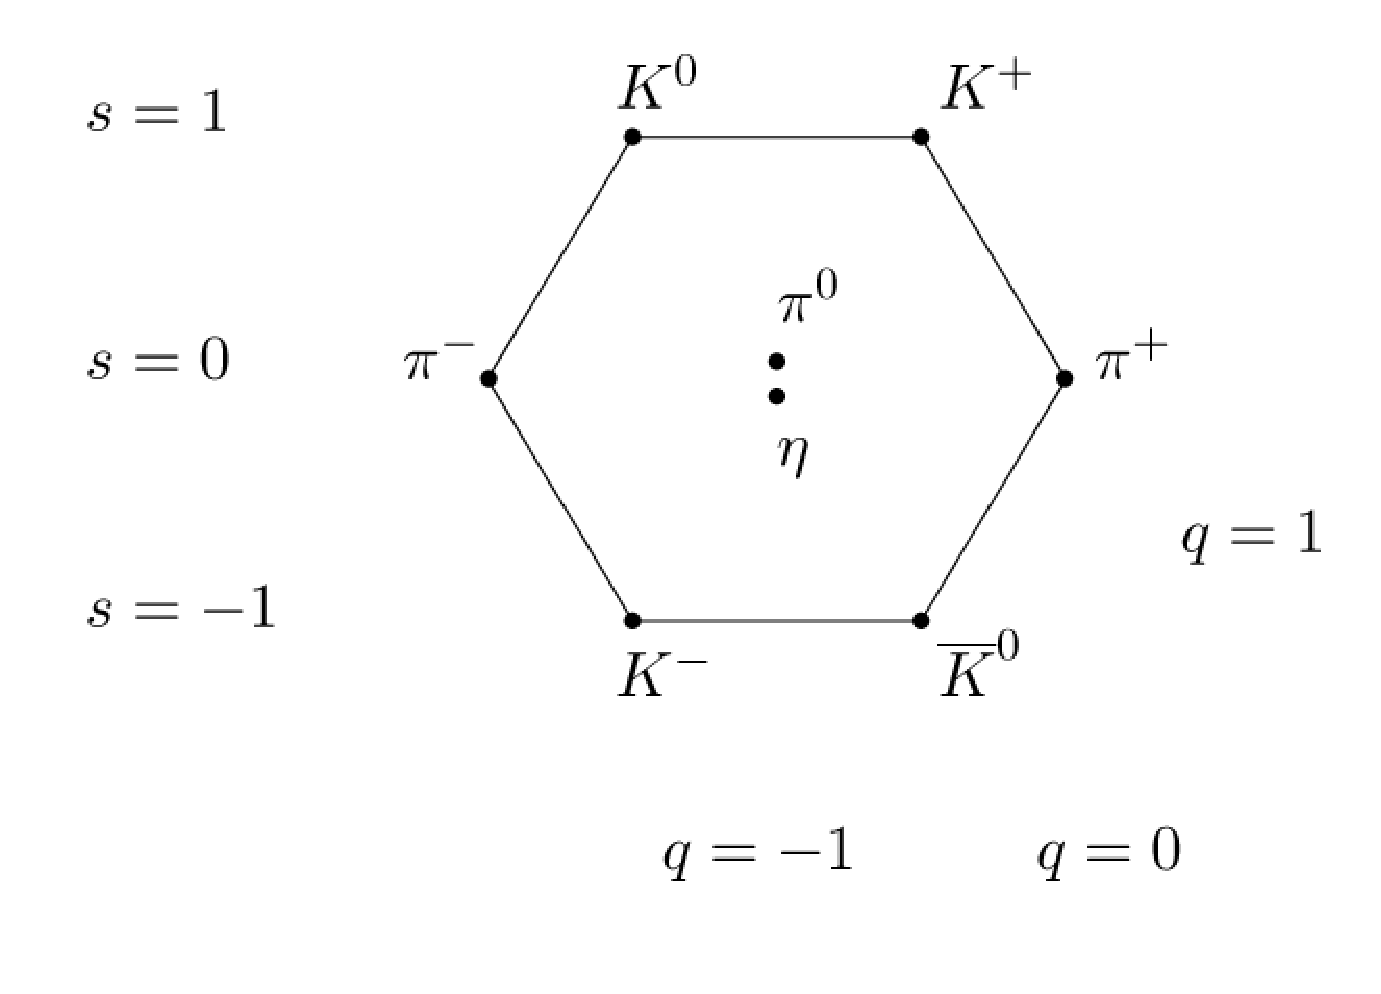
\includegraphics[width=0.45\textwidth]{figs/example/meson-octet}
    \caption{
        The lowest-energy meson octet.
    }
    \label{fig:meson-octet}
    \vspace{-0.3cm}
\end{wrapfigure}

Lorem ipsum dolor sit amet, consectetur adipisicing elit, sed do eiusmod tempor
incididunt ut labore et dolore magna aliqua. Ut enim ad minim veniam, quis
nostrud exercitation ullamco laboris nisi ut aliquip ex ea commodo consequat.
Duis aute irure dolor in reprehenderit in voluptate velit esse cillum dolore
eu fugiat nulla pariatur. Excepteur sint occaecat cupidatat non proident, sunt
in culpa qui officia deserunt mollit anim id est laborum.

Lorem ipsum dolor sit amet, consectetur adipisicing elit, sed do eiusmod tempor
incididunt ut labore et dolore magna aliqua. Ut enim ad minim veniam, quis
nostrud exercitation ullamco laboris nisi ut aliquip ex ea commodo consequat.
Duis aute irure dolor in reprehenderit in voluptate velit esse cillum dolore
eu fugiat nulla pariatur. Excepteur sint occaecat cupidatat non proident, sunt
in culpa qui officia deserunt mollit anim id est laborum.



